\chapter{How \textsc{Becca}'s feature creator works}
\label{perceiver_chapter}

A paper from the 2012 AAAI Spring Symposium on intelligent robots~\cite{rohrer12b} gives a full technical overview of \textsc{Becca}'s operation, but does not provide enough mathematical detail to fully describe its implementation. This section has those details, but only for the feature creator. A detailed mathematical description of the reinforcement learner is forthcoming

\textsc{Becca} creates features by 1) forming commonly co-active inputs into groups and 2) identifying observed patterns of activity within those groups. (See Figure~\ref{becca_feature_creator}.) For example, in prior work with image data \textsc{Becca} has formed nearby pixels (which are likely to be active at the same time more often than distant pixels) into groups and has chosen features within those pixels corresponding to oriented line segments and center-surround patterns.~\cite{rohrer11c} \textsc{Becca} requires no prior knowledge about the environment it is in, the nature of the experiences it is likely to have or the sensors that provide its input data. The one constraint it places on the world is that its inputs be real valued between zero and one, a constraint that is well suited to representing pixel values.

\begin{figure}
\centering
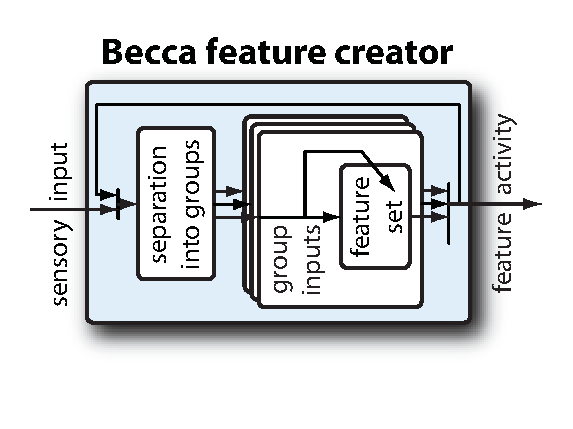
\includegraphics[height=7cm]{figs/becca_feature_creator.eps}
\caption{Block diagram of \textsc{Becca}'s feature creator.}
\label{becca_feature_creator}
\end{figure}


\section{Grouping}
The separation of input channels into groups is driven by how often each channel is co-active with each of the other channels. The goal of grouping is to find groups of input channels that tend to be mutually co-active. By virtue of their co-occurrence, activity in these channels is assumed to be not entirely independent.

When two channels are co-active, both have a value close to 1. Co-activity is conceptually similar to correlation, except that correlation is also influenced by co-{\em in}activity. Co-activity of channel A with channel B is defined as the probability that A is active, given that B is active. For binary inputs, this can be expressed as follows:

\begin{equation}
\kappa(A,B) = p(b|a)
\label{coactivity_def}
\end{equation}

where $\kappa(A,B)$ is the co-activity of channel A with channel B, and $p(b|a)$ is the probability that channel B is active, given that channel A is active. For the calculation of co-activity with real-valued inputs and its interpretation, see Section~\ref{coactivity_calc} at the end of this appendix. 

Co-activity between input channels can be described as a fully connected directed graph, which is most conveniently represented as a fully-populated matrix. The graph must be directed, because the co-activity of channel A with B is not in general equal to the co-activity of channel B with A. For instance, if channel A is fully active all the time and channel B is fully active only ten percent of the time, staying inactive the rest of the time, then from Equation~\ref{coactivity_def}, $\kappa(A,B) = 1$ but $\kappa(B,A) = 0.1$. Co-activity is estimated statistically, and the co-activity graph is updated incrementally at each time step. 

The co-activity of A with B,  $\kappa(A,B) $,  and the co-activity of B with A, $\kappa(B,A) $, can be combined to form the {\em mutual co-activity},  $\kappa_M(A,B) $ by taking the minimum of the two:

\begin{equation}
\kappa_M(A,B)   = \min(\kappa(A,B), \kappa(B,A)) 
\end{equation}

While co-activity is asymmetric, the mutual co-activity will always be symmetric. Mutual co-activity between input channels can be described as a fully connected, {\em un}directed graph. Mutual co-activity represents the extent to which two inputs are active at the same time, but does so in a way that does not overestimate the co-activity with very active inputs.

The process of grouping input channels can then be described as finding strongly interconnected subgraphs within the mutual co-activity graph. \textsc{Becca} does this using a greedy subgraph construction heuristic. Subgraph construction begins when one graph edge (the mutual co-activity of some input channel with another) exceeds a threshold, $C_1$. Those two input channels, say A and B, are added to the new group. Then, the channel with the highest average mutual co-activity with existing group members, $N_m$, is added:

\begin{equation}
N_m = \mbox{argmax}_{N}  \frac{\kappa_M(A,N) + \kappa_M(B, N)}{ 2}
\end{equation}

This agglomeration process continues until the mutual co-activity with the next candidate does not exceed another threshold, $C_2$.
Each time an input channel is added to a new group, its co-activity with all other channels is penalized by a factor of $e^{-C_3}$ from that point forward. This serves to limit the number of groups that a single channel can join. 

\section{Features}
Once a group has been formed, features can be created and evolved within it. \textsc{Becca} does this by randomly selecting features to start with, then incrementally modifying the features depending upon the patterns of activation observed within the group.

\subsection{Feature activity}

To be more precise, each input channel can be interpreted as a separate dimension in an $n$-dimensional input space, where $n$ is the total number of input channels. Groups then form $m$-dimensional subspaces of the input space, where $m$ is the number of input channels in a given group. At any time step, the input values to a group can be represented as a single point in that group's subspace. 

Features provide a way to coarsely discretize the inputs. \textsc{Becca} represents features as points on a unit sphere in a group's subspace. That is, a feature is a vector of the group's inputs, constrained to have a magnitude of one. In a group with $m$ inputs, empirical results suggest that $m/3$ (rounded upward) is a useful number of features to create. Many more than this creates an unnecessarily large feature set, increasing learning times, and many fewer than this does not provide a sufficiently rich feature set to allow high-performance learning. 

Before comparing it with features, the input is scaled:

\begin{equation}
\hat{s} = s  \frac{\max(s)} {|| s ||}
\end{equation}
 
This scaling gives the input two desirable properties: 
\begin{enumerate}
\item Assuming no component of the input is greater than 1, the scaled output will not be greater than 1.
\item The value of $\hat{s}$ will only be maximal (equal to 1) if one of one of its inputs is maximal. If this were not the case, inputs of many different magnitudes could produce the same scaled input.
\end{enumerate} 

In order to determine whether a scaled input is similar to existing features, a similarity metric is required. \textsc{Becca} uses the square of the magnitude of the projection of the scaled input onto a feature to determine its similarity. Because the feature magnitude is already known to be of magnitude 1, the similarity between input $s$ and feature $f$ can be calculated as follows:

\begin{equation}
\beta(\hat{s}, f) = (s \cdot f)^2
\end{equation}

The similarity, $\beta$, of an input with each feature in a group represents the {\em excitation} of each feature, the extent to which that input tends to excite activity within it. The similarity is treated like a vote. The feature receiving the highest vote is activated. However, the excitation of each feature is modulated by a fatigue factor, $\phi$, in the following way:

\begin{equation}
v =  \beta e^{-C_4 \phi}
\end{equation}

where $v$ is the vote of the input for the feature in question and $C_4$ is a user-selected constant with $0 < C_4 < 1$. 

The activity of each feature in the group, $a$, is determined by the votes:

\begin{eqnarray}
a_i& = &\beta_i  \qquad \mbox{for } i = \mbox{argmax}(v) \\
&= &0 \qquad \mbox{for all other } i
\end{eqnarray}

$\phi$ is an incrementally updated function of each feature's recent activity given by the following:

\begin{equation}
\phi_{t+1} = C_5 ( \phi_{t} + a_{t})
\end{equation}

where $C_5$ is a user selected constant between 0 and 1. When a feature is active, its fatigue factor increases, diminishing its tendency to be activated in subsequent time steps. When a feature is inactive, its fatigue factor decays over time, making it increasingly likely to be activated.

By holding most feature activities to zero, the group's features provide a sparse representation of its input subspace. The feature activities from all groups are combined to form the feature creator's output.

\subsection{Feature evolution}

At each time step features are also incrementally updated. The nature of the the updates is such that features evolve over time to represent the most commonly observed patterns in a group's inputs.

The active feature in each group is updated to resemble the set of inputs that resulted in its selection. The size of the update is determined by the feature activity and inhibition, $\gamma$, that the feature receives. Inhibition in turn is determined by the excitation of nearby features, and their similarity to the winning feature:

\begin{equation}
\gamma = e^{\sum_{j \neq i}{\beta(f_i, f_j)\beta(\hat{s}, f_j) C_6}}
\end{equation} 

where $f_i$ is the winning (active) feature, $\beta(f_i, f_j)$ is the similarity between the winning feature and each of the others, $\beta(\hat{s}, f_j) $ is the excitation of each of the other features, and $C_6$ is a user-selected constant with $0 < C_6 < 1$. 

The inhibition scales the update magnitude:

\begin{equation}
f_{i \mbox{ new}} = f_i + (f_i - \hat{s}) a_i \gamma C_7
\end{equation}

where $a_i$ is the feature activity of the winning feature, calculated above, and $C_7$ is a user-selected constant with $0 < C_7 < 1$. The newly adapted feature is then renormalized to ensure that it maintains a magnitude of 1:

\begin{equation}
 f_{i \mbox{ new}} = \frac{f_{i \mbox{ new}}}{|f_{i \mbox{ new}}|}
 \end{equation}
 
 Updating features in this way favors large updates when the winning feature is: 
 
 \begin{enumerate}
 \item far from other features
 \item far from the input that excited it
 \item strongly active
 \end{enumerate}
 
 Figure~\ref{feature_operation} summarizes the life of a feature set in pictorial form.

\begin{figure}
\centering
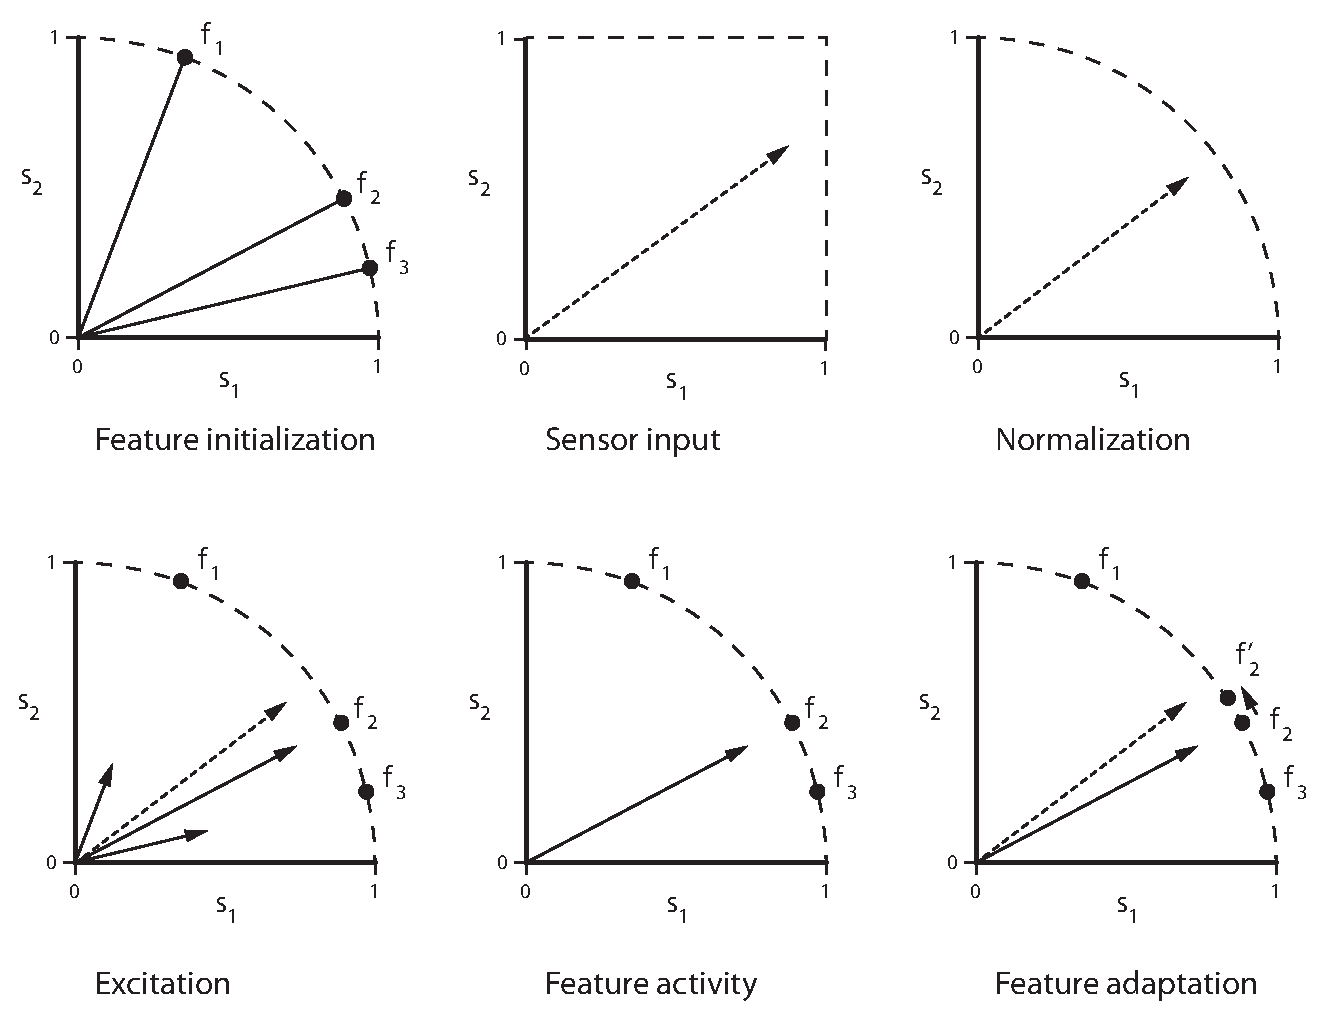
\includegraphics[height=9cm]{figs/feature_operation.eps}
\caption{The creation, operation, and evolution of features. In this example, a new group is created out of just two inputs, $s_1$ and $s_2$. Three initial features are chosen randomly from the set of positive unit vectors in the group space. On each subsequent time step, the values of $s_1$ and $s_2$ make a sensor input vector. Each time it is normalized, my the maximum possible magnitude of an input vector in the same direction. Then, it excites each of the features, according to its magnitude and its distance from them. The most excited feature is considered active for that time step, and the others are not. Finally, the winning feature migrates slightly toward the input that excited it.}
\label{feature_operation}
\end{figure}


\subsection{Computational requirements}

An important difference between \textsc{Becca} and other feature creation methods is that \textsc{Becca}'s feature creation and feature calculation operations occur on small subspaces of the input, rather than operating on the entire input space at once, as for instance principal components analysis does. This gives \textsc{Becca} the advantage of lower-order computational complexity for these operations: it is linear in the size of the input space rather than polynomial or exponential. This allows \textsc{Becca} to circumvent the curse of dimensionality to some extent and bodes well for its scalability to large problems. 

\section{Hierarchy, time, and domain knowledge} 

Three additional details of \textsc{Becca}'s operation are necessary to achieve its full capabilities. 

\begin{enumerate}

\item The first of these is the recurrent handling of its inputs and outputs. In addition to being \textsc{Becca}'s output, the feature activities at each time step are fed back into the grouper as the next time step's inputs. This allows features to be grouped with each other and other inputs to form new groups, in which higher-level features will be created. Due to its recurrent structure, this process may be repeated indefinitely, creating a hierarchical feature structure with an arbitrarily large number of hierarchy levels. In practice, new groups are only formed as often as co-activity dictates, which is limited by the structure inherent in the data.

\item The second detail is the temporal decay of inputs. After an input is active, its channel retains some residual activity on subsequent time steps, even if it is not externally stimulated. This decay is of a geometric nature, resulting in an exponential decay curve: 

\begin{equation}
s_{t+1} = C_8 s_t \mbox{,   \hspace{0.2in}  } 0 < C_8 < 1
\end{equation}

The result of this decay is that temporal aspects of data can be captured in the features. For instance, if input B is always active following input A, but never at the same time, retaining a decayed ghost of A's activity allows it to be correctly correlated with that of B to form a feature with temporal structure.

\item The third detail is the direct injection of user-created features to capture domain knowledge. As presented so far, \textsc{Becca} insists of deriving its own representation of the data from scratch. But in most applications, designers already have a pretty good guess about which features are likely to be informative in solving a given problem. \textsc{Becca} has a mechanism for incorporating engineered features as well. It looks for a vector of user-created feature primitives at each time step, in addition to raw sensor data. It handles the primitives differently that other inputs, concatenating them with the feature activities of all the created groups. As such, the primitives are both fed back as inputs, and included with the feature creator's output. The only constraint on primitives is that they also be real valued between zero and one. \textsc{Becca} handles both raw sensor inputs and feature primitives as fuzzy binary inputs, each indicating the graded presence of a certain attribute.

\end{enumerate}


\section{Co-activity}
\label{coactivity_calc}
\textsc{Becca}'s co-activity calculation is incremental, with the update method for real valued inputs given by the following:

\begin{equation}
\Delta\kappa(A, B) = C_9 a ( a b - \kappa(A, B) ) \mbox{,  \hspace{0.2in}  } 0 < C_9 < 1		
\label{coactivity_update}
\end{equation}

Where $\kappa$ is the co-activity, and $a$ and $b$ are the activity levels of channels A and B respectively. For values of $a$ and $b$ that remain constant over time, a convergence value for $\kappa(A, B)$ can be found from Equation~\ref{coactivity_update}. For the convergence criteria to be met, $\Delta\kappa(A, B) = 0$. That implies $a b - \kappa(A, B) = 0$ (assuming $a > 0$), giving the steady state value of

\begin{equation}
\kappa(A, B) = a b 
\end{equation}

The steady state value is symmetric in $a$ and $b$, even though the update rule is not. For constant-valued $a$ and $b$, $\kappa(A, B)$ and $\kappa(B, A)$ converge to the same value, but at different rates. 

Another instructive case is that of binary and stochastic inputs. Consider the independent input channels A and B such that

\begin{eqnarray}
A &|& p(a = 1) = 0.5 \mbox{, \hspace{0.2in}  } p(a = 0) = 0.5\\
B &|& p(b = 1) = 0.1 \mbox{, \hspace{0.2in}  } p(a = 0) = 0.9 	
\end{eqnarray}

The structure of the update rule guarantees that $\Delta\kappa(A, B) = 0$ when $a = 0$ , meaning that $\kappa(A, B)$ will not be modified in any way. It will only be updated when $a = 1$. The steady state value for $\kappa(A, B)$ can then be calculated by observing that when $a = 1$, the update rule reduces to 

\begin{equation}
\Delta \kappa(A, B) = b - \kappa(A, B)  
\end{equation}

The fact that B is independent from A implies that $\kappa(A, B)$ will converge to the mean of $b$, 0.1 . Following a similar set of calculations, it can be shown that $\kappa(B, A)$ converges to 0.5 . This illustrates the effect of asymmetry in the update rule on non-constant input values. The results can be verbalized as �Channel A is co-active with Channel B ten percent of the time, but Channel B is co-active with Channel A fifty percent of the time.� An intuitive metaphor is that of restless kindergarteners at nap time. The teacher has told all the children to lay still and close their eyes, but unable to help themselves, some of the children occasionally peek. $\kappa(A, B)$ is the probability that, when child A peeks, she will see child B's eyes open and vice versa.

One final observation about $\kappa(A, B)$ is that it is bounded both above and below by the product of $a$ and $b$. Since $0 \leq a \leq 1$ and $0 \leq b \leq 1$ ,  it follows that 

\begin{eqnarray}
0 \leq&ab&  \leq 1 \\
0 \leq&\kappa(A, B)&  \leq 1 
\end{eqnarray}
